\begin{figure}[H]
  \centering
  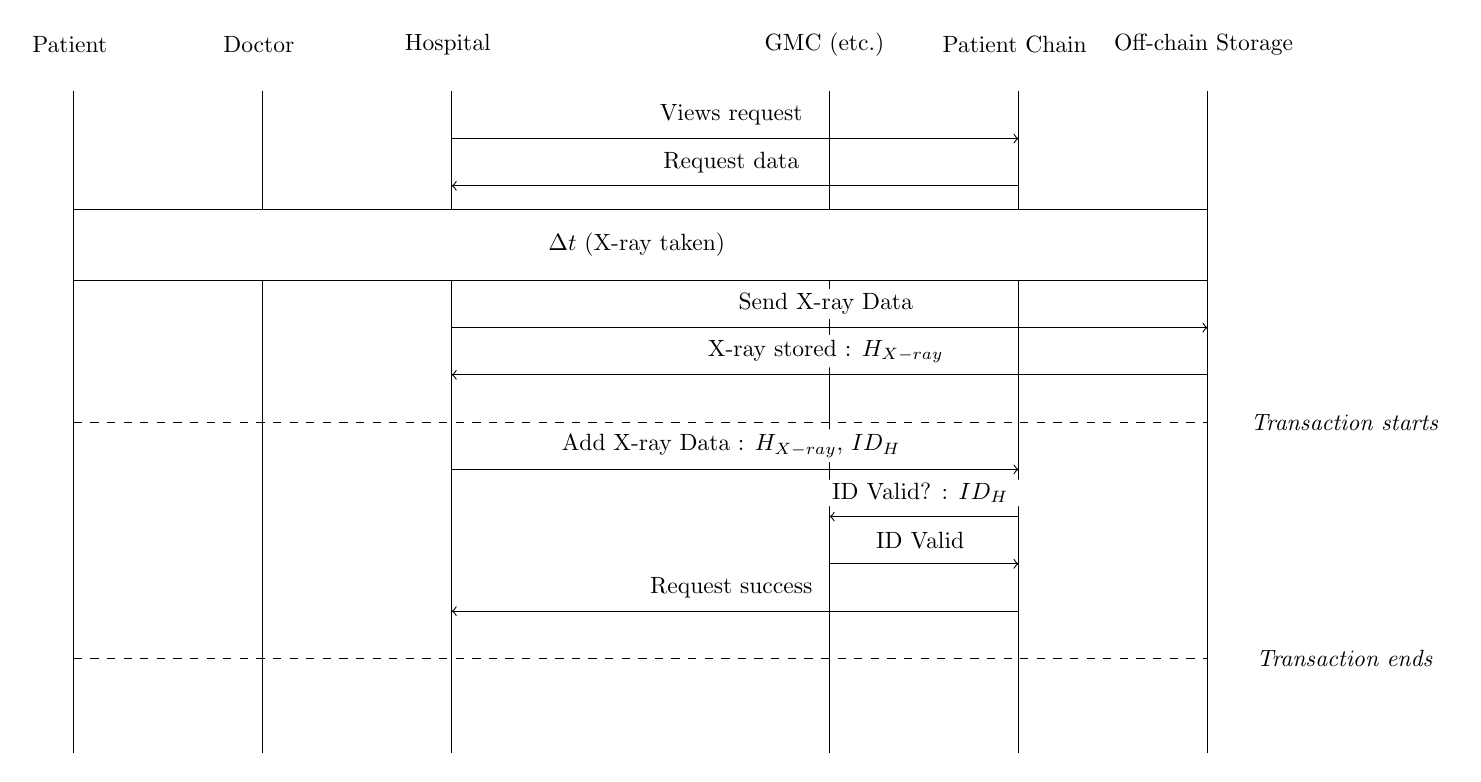
\begin{tikzpicture}[scale = 0.6, every node/.style={scale = 0.85}, every node/.append style={fill = white, rounded corners = 2pt, inner sep = 2pt, align = center}]

  % Lines
  \draw (4, 6) -- (4, 20);
  \draw (8, 6) -- (8, 20);
  \draw (12, 6) -- (12, 20);
  \draw (20, 6) -- (20, 20);
  \draw (24, 6) -- (24, 20);
  \draw (28, 6) -- (28, 20);

  % Headings
  \node at (4, 21) { Patient };
  \node at (8, 21) { Doctor };
  \node at (12, 21) { Hospital };
  \node at (20, 21) { GMC (etc.) };
  \node at (24, 21) { Patient Chain };
  \node at (28, 21) { Off-chain Storage };

  % Arrows
  \node at (18, 19.5) { Views request };
  \draw [ -> ] (12, 19) -- (24, 19);

  \node at (18, 18.5) { Request data };
  \draw [ -> ] (24, 18) -- (12, 18);

  \draw[fill = white] (4, 17.5) rectangle (28, 16);
  \node at (16, 16.75) { $\Delta t$ (X-ray taken) };

  \node at (20, 15.5) { Send X-ray Data };
  \draw [ -> ] (12, 15) -- (28, 15);

  \node at (20, 14.5) { X-ray stored \checkmark : $H_{\text{X-ray}}$ };
  \draw [ -> ] (28, 14) -- (12, 14);

  \node at (31, 13) { \textit{Transaction starts} };
  \draw [ dashed ] (4, 13) -- (28, 13);

  \node at (18, 12.5) { Add X-ray Data : $H_{\text{X-ray}}$, $ID_{H}$ };
  \draw [ -> ] (12, 12) -- (24, 12);

  \node at (22, 11.5) { ID Valid? : $ID_{H}$ };
  \draw [ -> ] (24, 11) -- (20, 11);

  \node at (22, 10.5) { ID Valid \checkmark };
  \draw [ -> ] (20, 10) -- (24, 10);

  \node at (18, 9.5) { Request success };
  \draw [ -> ] (24, 9) -- (12, 9);

  \node at (31, 8) { \textit{Transaction ends} };
  \draw [ dashed ] (4, 8) -- (28, 8);

  \end{tikzpicture}
  \caption{
    Patient visits hospital to have X-ray taken
  }{
    The hospital views the request made by the doctor (that relates to the appointment). Upon viewing the data, they take the X-ray. The X-ray data is sent to some off-chain storage and the address (potentially the hash of the content) is returned. This hash is then added by the hospital to the patient's record as X-ray data.
  }
  \label{fig:user_story_02}
\end{figure}
